% !TEX TS-program = pdflatex
% !TEX encoding = UTF-8 Unicode

\documentclass{article}
\usepackage{kotex, ulem}
\usepackage{graphicx}
\usepackage{subfigure}
\usepackage{amsmath}
\usepackage{kmath}
\usepackage{color}
\usepackage[a4paper,left=30mm,right=30mm,top=23mm,bottom=25mm]{geometry}



\begin{document}

\title{프로그래밍 언어 HW0}
\author{B811056 노이진}
\date{2021-03-19}
\maketitle

\section{자기소개}
 안녕하세요. 저는 홍익대학교 컴퓨터공학과 18학번에 재학 중인 23살 노이진입니다.
\section{수식작성}

\colorbox{black}{\textcolor{white}{\#18}}  \textbf{\uline{평균변화율}}\newline
$\Diamondblack$ x의 증분과 y의 증분

 함수 $f(x)$에서 $x$의 값이 $a$에서 $b$까지
 
 변할 때, 함수값 $y$는 $f(a)$에서 $f(b)$
 
 까지 변한다.
 
  - $x$의 값의 변화량 $b-a$를 $x$의 증분
  
  \, 이라 하고, $\Delta$$x=b-a$
  
  - $y$의 값의 변화량 $f(b)-f(a)$를 
  
  \, $y$의 증분이라 하고,
  
  \, $\Delta$$y=f(b)-f(a)$\newline
$\Diamondblack$ 평균변화율

- $x$의 증분 $\Delta$$x$에 대한 $y$의 증분 $\Delta$$y$

\, 의 비


- $\cfrac{\Delta y}{\Delta x}$
$=$
$\cfrac{f(b)-f(a)}{b-a}$
$=$
$\cfrac{f(a+\Delta x)-f(a)}{\Delta x}$

\, (단, $\Delta$$x=b-a$)

\section{가장 좋아하는 그림}
\subsection{자신을 나타낼 수 있는 사진}
\begin{figure}[h]
\centering
   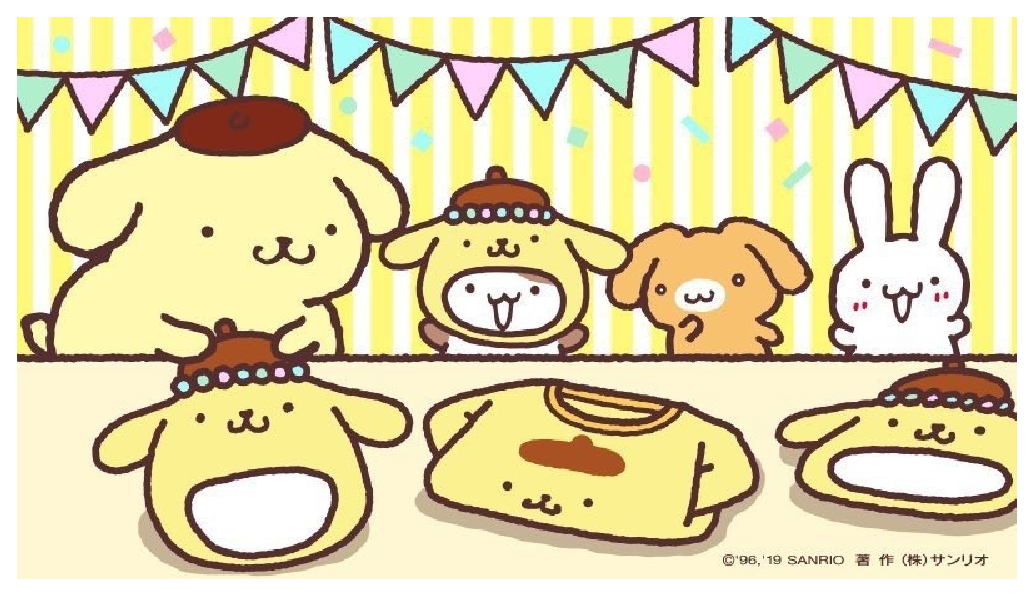
\includegraphics[width=10cm]{image1}
\caption{폼폼푸린}
\label{3.1}
\end{figure}

Fig 3.\ref{3.1}은 내가 가장 좋아하는 캐릭터인 폼폼푸린이다. 폼폼푸린은 골든 리트리버이고 다른 동물 친구들이 많다. 평소 폼폼푸린과 관련된 제품을 항상 곁에 두고 지내기 때문에 나를 나타내는 사진으로 선택했다.

\subsection{좋아하는 연예인 사진}
\begin{figure}[h]
    \centering
    \begin{subfigure}
        \centering
        \includegraphics[width=0.92\linewidth]{image2.eps}  
        \label{sub-first}
    \end{subfigure}
    \begin{subfigure}
        \centering
        
\includegraphics[width=3.8cm]{image3}  
        \label{sub-second}
    \end{subfigure}
    \begin{subfigure}
        \centering
        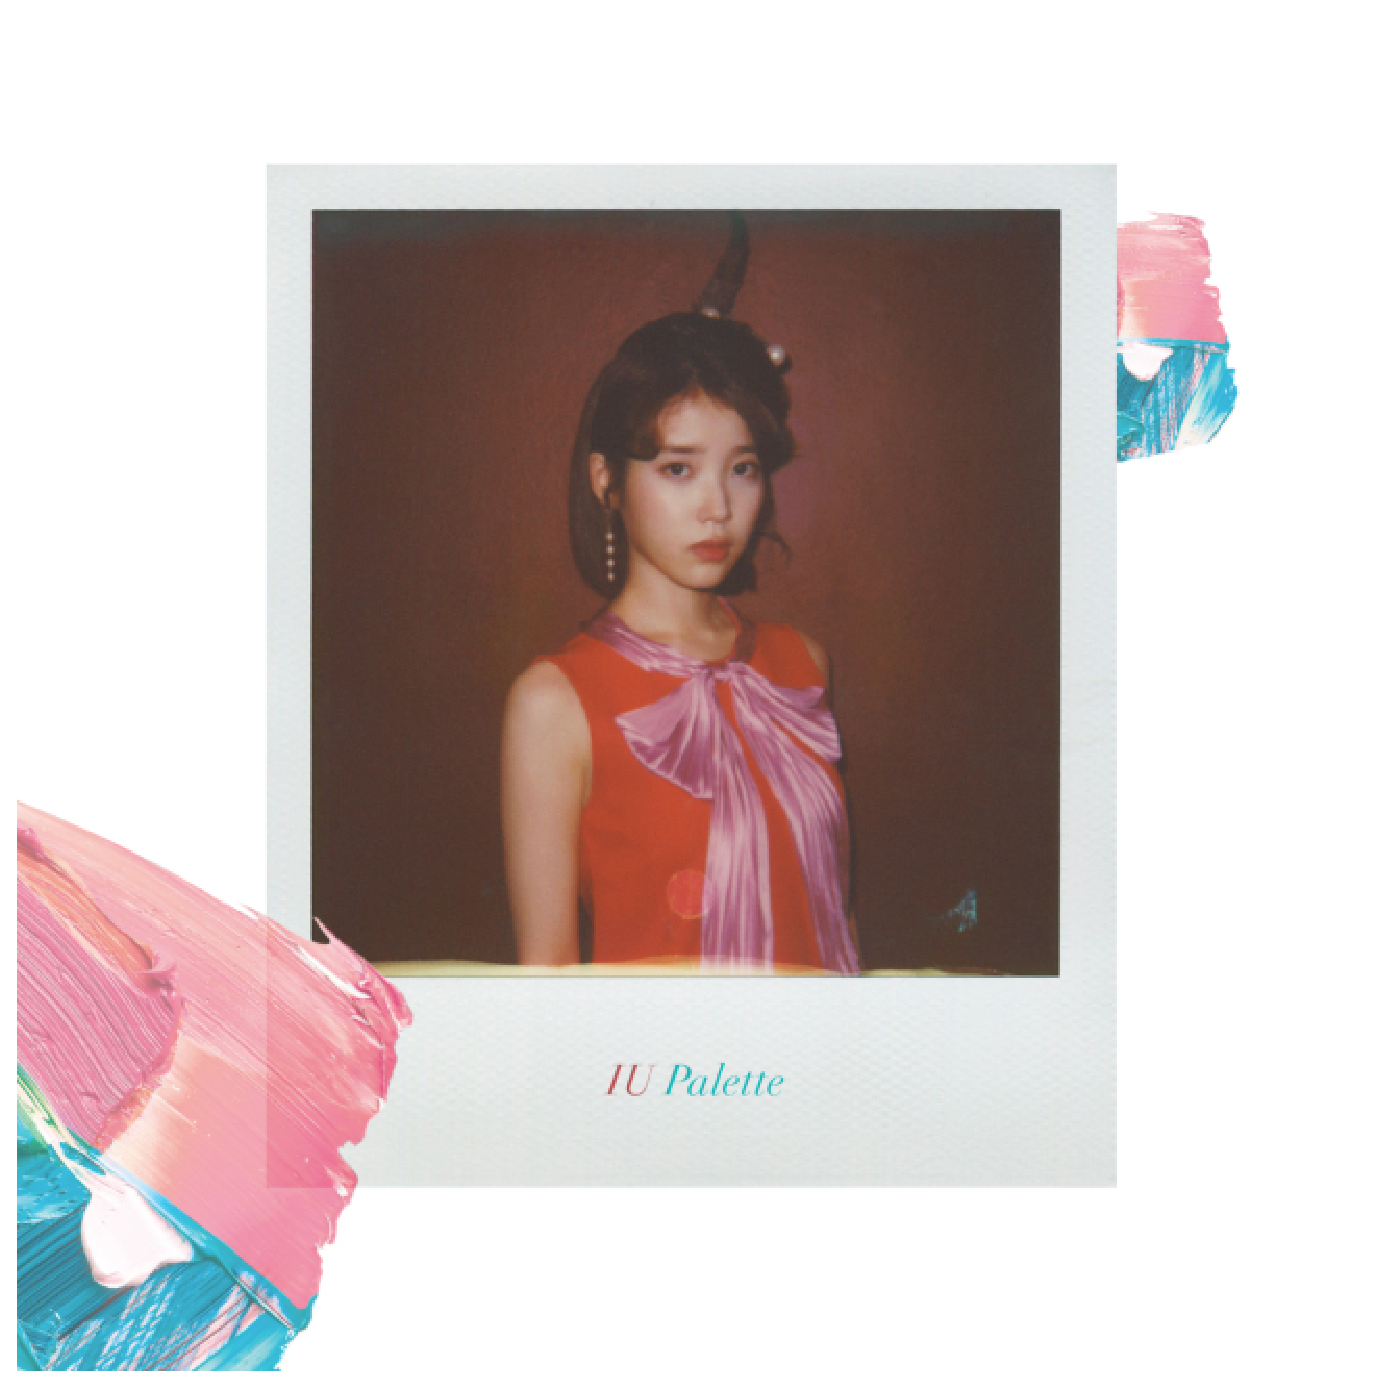
\includegraphics[width=4.3cm]{image5}  
        \label{sub-third}
    \end{subfigure}
    \begin{subfigure}
        \centering
        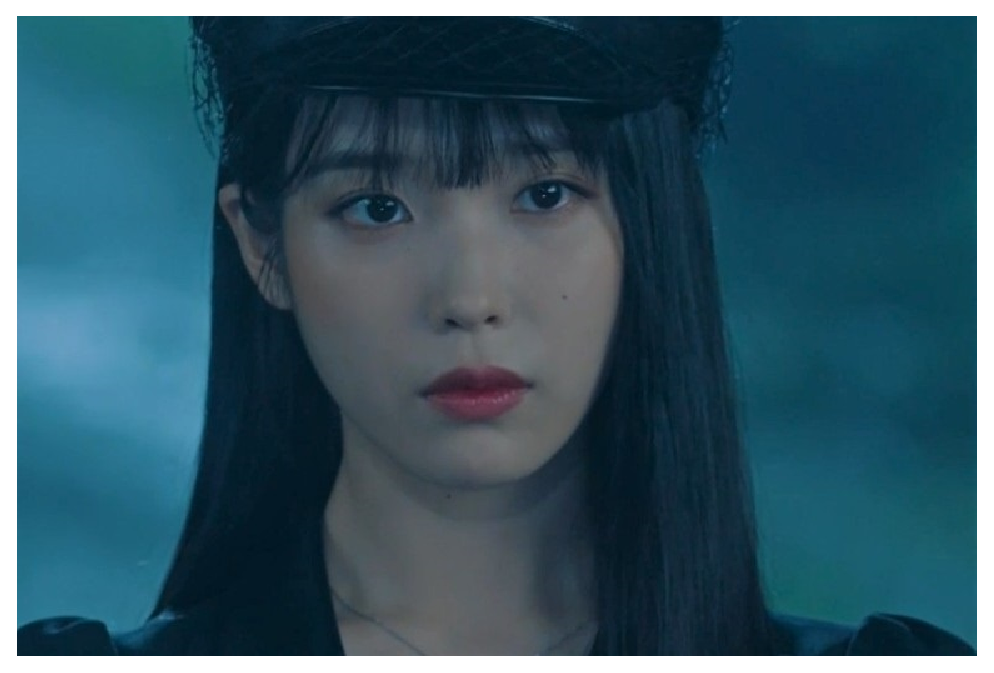
\includegraphics[width=5cm]{image4}  
        \label{sub-fourth}
    \end{subfigure}
    \caption{아이유}
    \label{3.2}
\end{figure}

Fig 3.\ref{3.2}는 가수이자 연기자로 활동 중인 아이유의 사진이다. 나는 특히 호텔 델루나 때의 아이유를 좋아하기 때문에 그 때의 사진을 심도있게 골라보았다. 가장 마음에 드는 사진을 가장 크게 배치했고, 아래줄 중앙에는 정규 4집 앨범인 palette의 표지도 넣었다. palette는 타이틀 곡인 팔레트뿐만 아니라 수록곡들도 모두 완벽해서 가장 좋아하는 앨범이다.
\end{document}

